\documentclass[14pt]{extarticle} 
\usepackage{amsmath,mathtools,amsfonts,amsthm,amssymb,hyperref}
\usepackage{wasysym,parskip,bookmark,geometry,graphicx,float}
\hypersetup{colorlinks,allcolors=blue,linktoc=all}
\newtheorem{defn}{Definition}
\newtheorem{thm}{Theorem}
\newtheorem{claim}{Claim}
\newtheorem{lemma}{Lemma}
\geometry{a4paper} 
\geometry{margin=0.5in} 
\title{Solutions to Math for CS 2015/2019 ``In-Class Problems Week 1, Wed.''}
\author{https://github.com/spamegg1}
\begin{document}
\maketitle
\tableofcontents
\section{Problem 1.}
This regards the ``visual proof'' of the Pythagorean Theorem: $a^2 + b^2 = c^2$.

\subsection{(a)}

You will first arrange the square and four triangles so they form a $c \times c$ square. From this arrangement you will see that the square is $(b - a) \times (b - a)$.

\begin{proof}
We can do this as follows:
\begin{figure}[ht!]
\centering
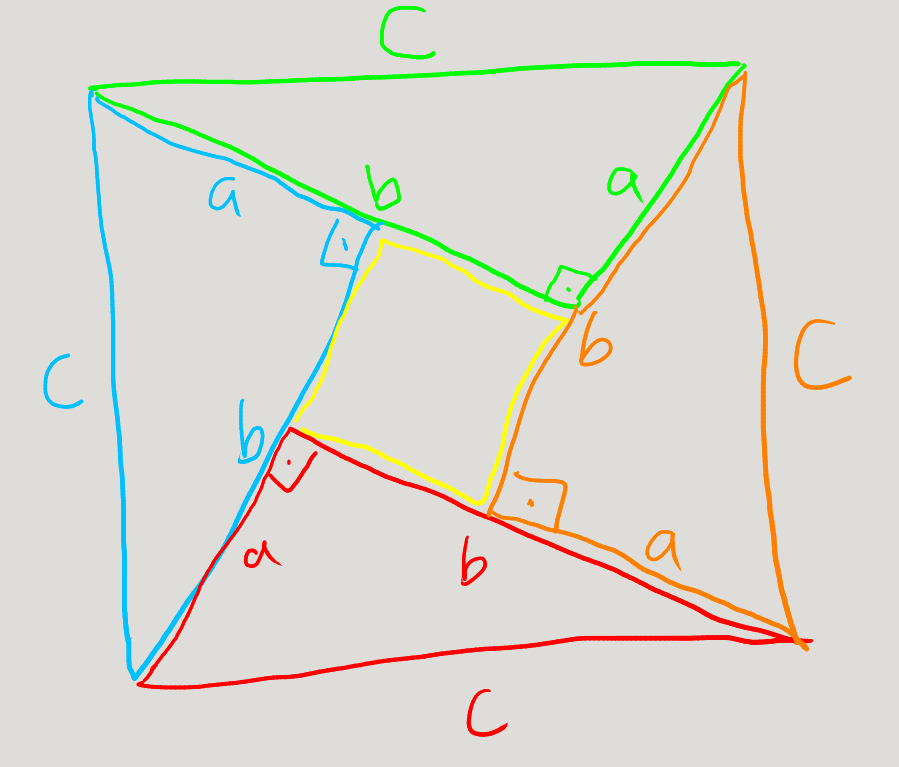
\includegraphics[scale=0.25]{onesquare.png}
\end{figure}
\end{proof}

\subsection{(b)}

You will then arrange the same shapes so they form two squares, one $a \times a$ and the other $b \times b$.

\begin{proof}
We can do this as follows:
\begin{figure}[ht!]
\centering
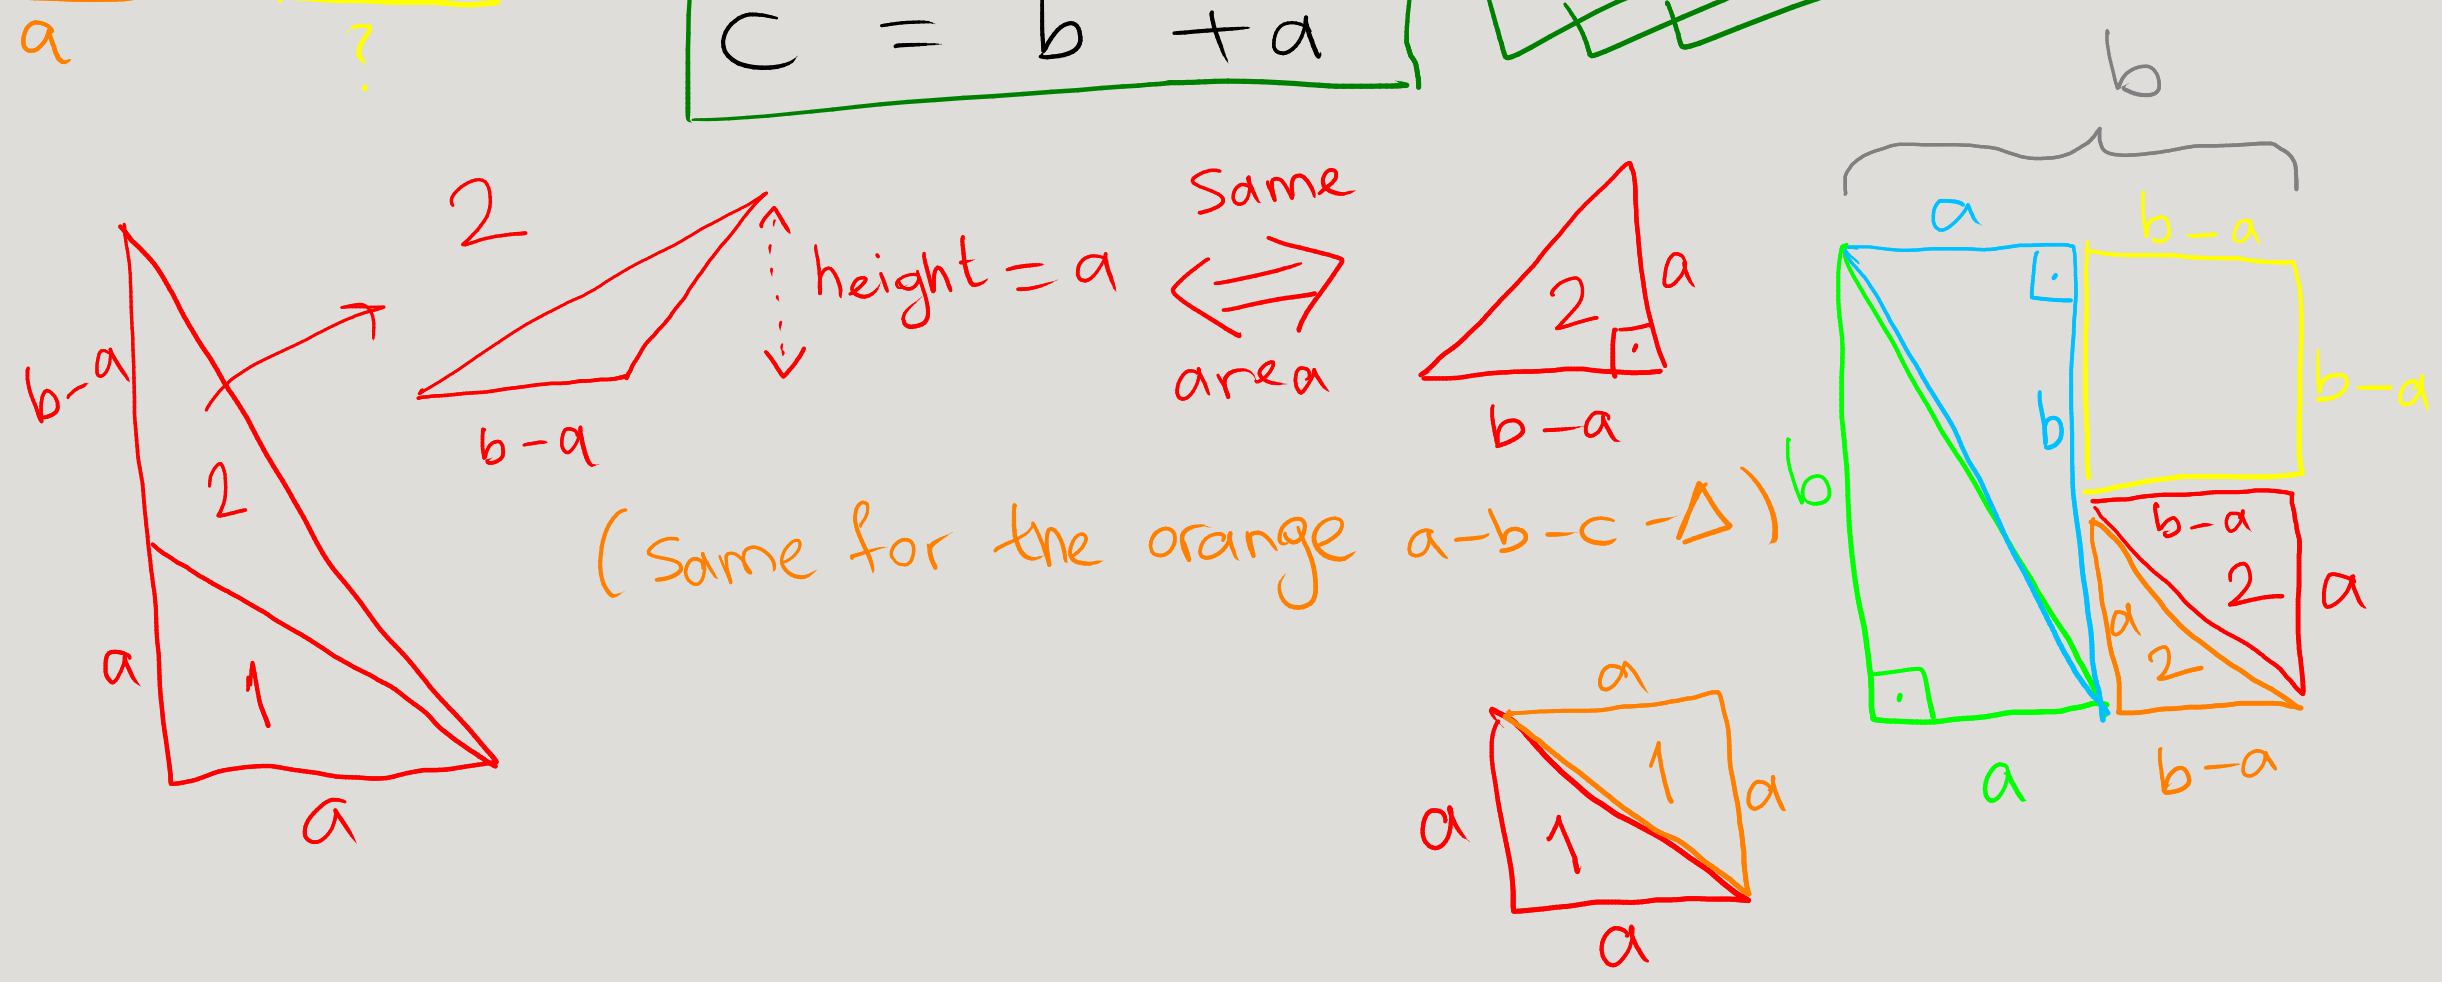
\includegraphics[scale=0.20]{twosquares.png}
\end{figure}
\end{proof}

\subsection{(c)}

One concern is that there might be something special about the shape of these particular triangles and square that makes the rearranging possible -- for example, suppose $a = b$?

How would you respond to this concern?

\begin{proof} 
There are 3 possibilities for the relation between $a$ and $b$:

{\bf Case 1.} $a < b$. This corresponds to our picture proof above.

{\bf Case 2.} $b < a$. In this case, we could simply switch the roles of $a$ and $b$. In other words, we can simply ``rename'' our variables. We can rename $a$ to $b$, and $b$ to $a$. Then we end up with Case 1 above.

{\bf Case 3.} $a = b$. In this case we can give an explanation that the yellow square with sides $b - a$ shrinks to nothing. Or we can give the picture proof directly:

\begin{figure}[ht!]
\centering
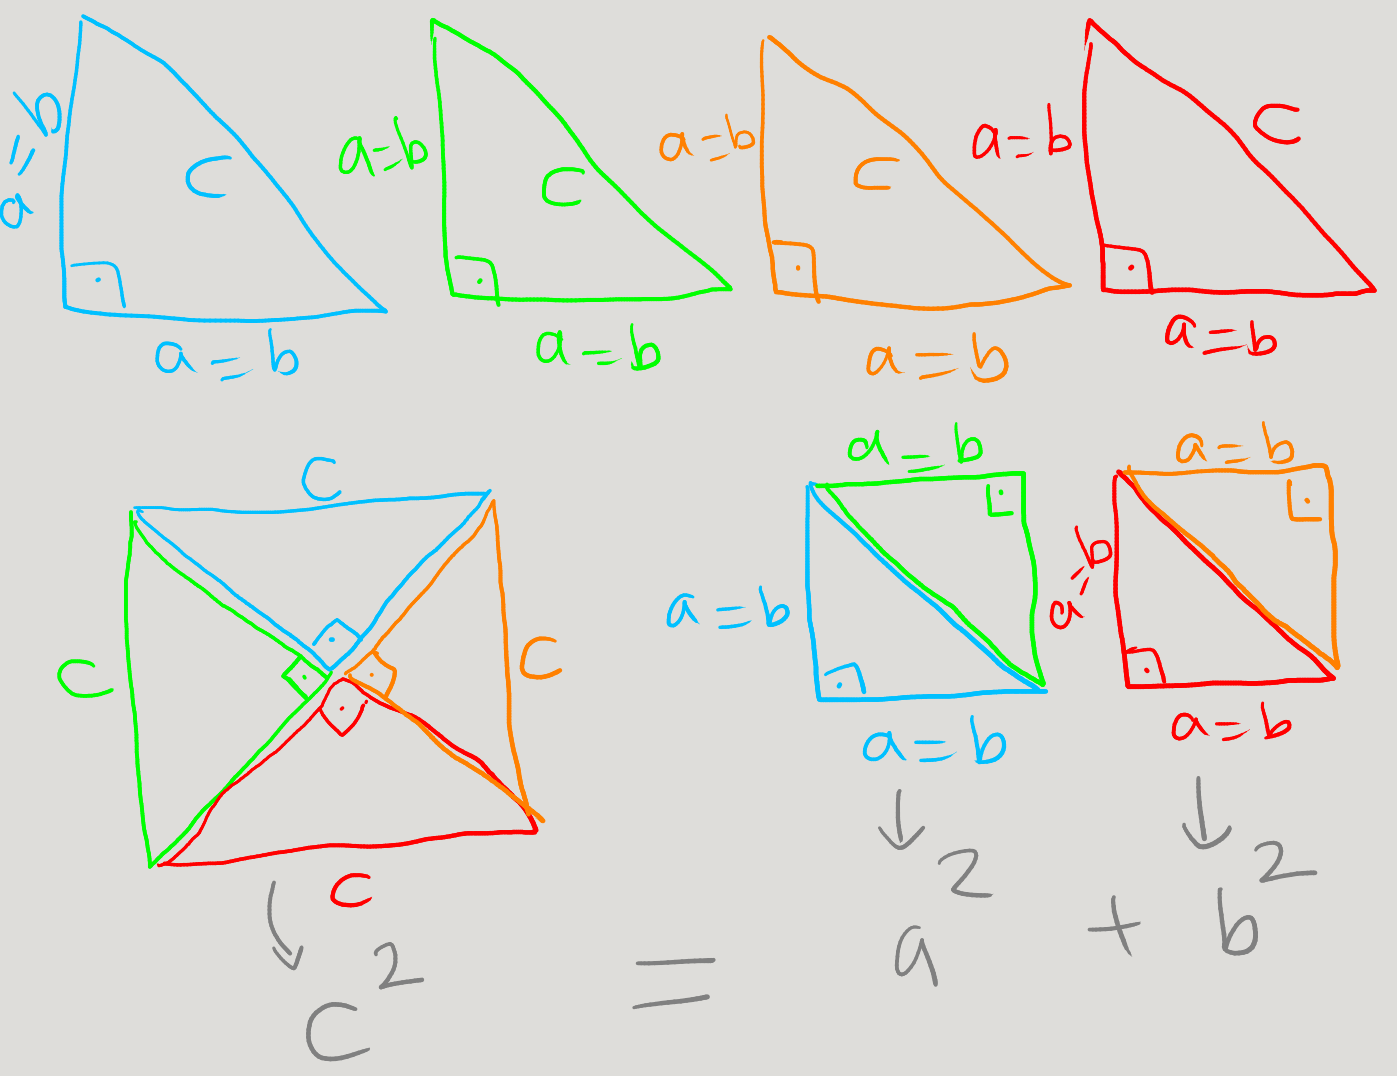
\includegraphics[scale=0.25]{aequalsb.png}
\end{figure}
\end{proof}

\subsection{(d)}

Another concern is that a number of facts about right triangles, squares and lines are being implicitly assumed in justifying the rearrangements into squares. Enumerate some of these assumed facts.

\begin{proof}
We are assuming that:

The area of a triangle with base length $b$ and height $h$ is $b \cdot h / 2$;

The area of a right triangle with right sides of lengths $a$ and $b$ is $a\cdot b / 2$ (which is a special case of the above);

The areas of two triangles with the same base length and same height are equal, regardless of the shapes of the triangles;

If $a < b$, we can take a line segment of length $b$ and split it into two parts of lengths $a$ and $b - a$;

The sum of internal angles of a triangle is 180 degrees (and the sum of the two non-right angles of a right-triangle is 90 degrees);

A triangle (similarly, a square) can be rotated, moved, shifted while keeping all the internal angles and side lengths the same;

and probably some other facts that are too difficult to put into words (without going all the way down to Euclid's Five Axioms of Plane Geometry).
\end{proof}

\section{Problem 2.}
This regards the bogus proof:

$$
1 = \sqrt{1} = \sqrt{(-1)(-1)} = \sqrt{-1}\sqrt{-1} = (\sqrt{-1})^2 = -1
$$

\subsection{(a)}

Precisely identify and explain the mistake(s) in this bogus proof.

\begin{proof}
The issue is with the step $\sqrt{(-1)(-1)} = \sqrt{-1}\sqrt{-1}$. We are assuming a hidden property: $\sqrt{ab} = \sqrt{a}\cdot\sqrt{b}$.
\end{proof}

\subsection{(b)}

Prove (correctly) that if $1 = -1$, then $2 = 1$.

\begin{proof}
In the video and slides, Prof. Meyer gives a correct proof that: if $1 = -1$ then $2 = 1$. It goes like this:

(1) Assume $1 = -1$. 

(2) Dividing (1) by 2, we get $\frac{1}{2} = -\frac{1}{2}$

(3) Adding $3/2$ to both sides of (2) we get $\frac{1}{2}  + \frac{3}{2} = -\frac{1}{2} + \frac{3}{2}$

(4) Rewriting (3) we get $2 = 1$.
\end{proof}

\subsection{(c)}

Every positive real number, $r$, has two square roots, one positive and the other negative. The standard convention is that the expression $\sqrt{r}$ refers to the positive square root of $r$. Assuming familiar properties of multiplication of real numbers, prove that for positive real numbers $r$ and $s$,
$$
\sqrt{rs} = \sqrt{r}\sqrt{s}
$$

{\bf Solution.} For the sake of clarity, let's define the positive square root:

\begin{defn} 
Assume $r > 0$ is a real number. A {\bf positive square root of} r is a real number $x > 0$ with the property $x^2 = r$.
\end{defn}

So the problem gives us the fact that positive square roots {\it exist} and they are {\it unique}:

\begin{thm}
For every real number $r > 0$ there exists a unique positive square root of $r$, denoted by $\sqrt{r}$.
\end{thm}

Now solving the problem:
\begin{proof}
\begin{align*}
rs & = rs &\text{(true by tautology)}\\
(\sqrt{rs})^2 & =  (\sqrt{r})^2(\sqrt{s})^2 &\text{(by the existence of positive square roots)}\\
(\sqrt{rs})^2 & = (\sqrt{r}\sqrt{r})(\sqrt{s}\sqrt{s}) &\text{(by definition of squares)}\\
(\sqrt{rs})^2 & = \sqrt{r}(\sqrt{r}\sqrt{s})\sqrt{s} &\text{(by associativity of multiplication)}\\
(\sqrt{rs})^2 & = \sqrt{r}(\sqrt{s}\sqrt{r})\sqrt{s} &\text{(by commutativity of multiplication)}\\
(\sqrt{rs})^2 & = (\sqrt{r}\sqrt{s})(\sqrt{r}\sqrt{s}) &\text{(by associativity of multiplication)}\\
(\sqrt{rs})^2 & = (\sqrt{r}\sqrt{s})^2 &\text{(by definition of squares)}\\
\sqrt{rs} &=  \sqrt{r}\sqrt{s}  &\text{(by the uniqueness of positive square roots)}\\
\end{align*}
\end{proof}

\section{Problem 3}

Identify exactly where the bugs are in each of the following bogus proofs.

\subsection{(a)}

{\bf Bogus claim.} $1/8 > 1/4$.

{\it Bogus proof.}
\begin{align}
3 & > 2 \\
3\log_{10}(1/2) & > 2\log_{10}(1/2)\\
\log_{10}(1/2)^3 & > \log_{10}(1/2)^2\\
(1/2)^3 &> (1/2)^2 \\
1/8 &> 1/4
\end{align}

\begin{proof}
The problem is on Step (2). We are multiplying both sides of a true inequality $3 > 2$ with the same number $\log_{10}(1/2)$. According to the rules of real numbers, if $r, s$ and $t$ are real numbers with $r > s$, and if $t > 0$ then $rt > st$; if $t < 0$ then $rt < st$. 

So the inequality should stay the same if that number is positive; it should reverse if the number is negative. The issue is that $\log_{10}(1/2)$ is actually negative! It's around $-0.3$. So the inequality should reverse directions, but in the bogus proof it does not.
\end{proof}

\subsection{(b)}

{\it Bogus proof.}
$$
1 \cent = \$ 0.01 = (\$ 0.1)^2 = (10\cent)^2 = 100\cent = \$1
$$

\begin{proof}
Let's try to give an accurate calculation, by using the fact that $\$1 = 100\cent$ and squaring the units along with the numbers (like you would in physics). This one is certainly true:

$$
1 \cent = \$ 0.01
$$

How about $(\$ 0.1)^2$?

$$
(\$ 0.1)^2 = (100\cent \cdot 0.1)^2 = (10\cent)^2 = 100\cent^2
$$

So as you can see, the second step is already wrong. $1\cent$ is not the same as $100\cent^2$. 
Step 3 seems true:

$$
(\$ 0.1)^2 = 100\cent^2 = (10\cent)^2
$$

Step 4 is clearly wrong:

$$
(10\cent)^2 = 100\cent^2 \neq 100\cent
$$

Step 5 is correct:

$$
100\cent = \$1
$$
\end{proof}

\subsection{(c)} 

{\bf Bogus claim.} If $a$ and $b$ are two equal real numbers, then $a = 0$.

{\it Bogus proof.}
\begin{align}
a &=b  \\
a^2 &= ab\\
a^2-b^2 &= ab-b^2\\
(a-b)(a+b) &= b(a-b)\\
a+b &= b\\
a &= 0
\end{align}

\begin{proof}
The only wrong step is going from (9) to (10): we are dividing both sides by zero! Because $a - b= 0$.
\end{proof}

\section{Problem 4}

It’s a fact that the Arithmetic Mean is at least as large as the Geometric Mean, namely,
$$
\frac{a+b}{2} \geq \sqrt{ab}
$$

{\it Bogus proof.}
\begin{align}
\frac{a+b}{2} &\geq^?\sqrt{ab}  \\
a+b &\geq^? 2\sqrt{ab} \\
a^2+2ab+b^2 &\geq^? 4ab\\
a^2-2ab+b^2 &\geq^? 0\\
(a-b)^2 &\geq^? 0 \text{ true}
\end{align}

\begin{proof}
So it proves (12) $ \implies $ (13) $ \implies $ (14) $ \implies $ (15) $ \implies $ (16), which is true, but we don't know if (12) is true or not. We assumed what we were supposed to prove (12), then did a bunch of correct steps, and reached a true statement at the end. But that doesn't prove anything! 

All the statements \textit{happen to be true} in this case, but this is not shown by the implications in this bogus proof (because we don't know if the initial assumption in (12) is true or not). Remember from before, that if you start from a false assumption, such as $1 = -1$, then you can ``prove'' pretty much anything (like $2 = 1$).

But if we prove all the implications in reverse, the proof is correct! We can start with the true statement (16). Then apply correct steps going backwards. Then we reach (12), which then must also be true.

There is a bit of an issue that we need to be careful with: proving the implication (14) $\implies$ (13) involves taking square roots of both sides. We have to know that both $a^2 + 2ab + b^2$ and $4ab$ are nonnegative (can't take square root of a negative number), and we also have to use the Calculus fact that the square root function is increasing (so that the inequality $\geq$ is preserved after taking square roots).
\end{proof}

\section{Problem 5}
This is optional (thankfully) and it's definitely not useful, helpful or educational. It's just crazy nonsense because it mixes in vague non-logical non-mathematical notions like surprise, expectations, future etc. Just skip this and don't waste your time. Thinking about \href{https://en.wikipedia.org/wiki/Unexpected_hanging_paradox}{wordy English paradoxes} will rot your logical thinking brain. 
\end{document}
